\documentclass{article}
\usepackage[utf8]{inputenc}
\usepackage{listings}
\usepackage{multimedia} % to embed movies in the PDF file
\usepackage{graphicx}
\usepackage{comment}
\usepackage[english]{babel}
\usepackage{amsmath}
\usepackage{amsfonts}
\usepackage{subfigure}
\usepackage{wrapfig}
\usepackage{multirow}
\usepackage{tikz}
\usepackage{verbatim}

\newtheorem{theorem}{Theorem}[section]
\newtheorem{lemma}[theorem]{Lemma}
\newtheorem{corollary}[theorem]{Corollary}
%\newtheorem{algorithm}[theorem]{Algorithm}
\newtheorem{remark}[theorem]{Remark}
\newenvironment{proof}{\noindent {\bf Proof:} }{\hfill $\Box$ \\[2ex] }
\newenvironment{keywords}{\begin{quote} {\bf Key words} }
                         {\end{quote} }
\newenvironment{AMS}{\begin{quote} {\bf AMS subject classifications} }
                         {\end{quote} }


\newcommand{\eref}[1]{\mbox{\rm(\ref{#1})}}
\newcommand{\tref}[1]{\mbox{\rm\ref{#1}}}
\newcommand{\set}[2]{\left\{ #1 \; : \; #2 \right\} }
\newcommand{\deq}{\raisebox{0pt}[1ex][0pt]{$\stackrel{\scriptscriptstyle{\rm def}}{{}={}}$}}

\newcommand {\DS} {\displaystyle}

\newcommand{\real}{\mathbb{R}}
\newcommand{\compl}{\mathbb{C}}



\newcommand {\half} {\mbox{$\frac{1}{2}$}}
\newcommand{\force}{{\mathbf{f}}}
\newcommand{\strain}{{\boldsymbol{\varepsilon}}}
\newcommand{\stress}{{\boldsymbol{\sigma}}}
\renewcommand{\div}{{\boldsymbol{\nabla}}}

\newcommand {\cA} {{\cal A}}
\newcommand {\cB} {{\cal B}}
\newcommand {\cC} {{\cal C}}
\newcommand {\cD} {{\cal D}}
\newcommand {\cE} {{\cal E}}
\newcommand {\cL} {{\cal L}}
\newcommand {\cP} {{\cal P}}
\newcommand {\cQ} {{\cal Q}}
\newcommand {\cR} {{\cal R}}
\newcommand {\cV} {{\cal V}}
\newcommand {\cW} {{\cal W}}
\newcommand {\CH} {{\cal H}}
\newcommand {\CS} {{\cal S}}


\newcommand{\bzero}{\mathbf{0}}
\newcommand{\ba}{\mathbf{a}}
\newcommand{\bb}{\mathbf{b}}
\newcommand{\bc}{\mathbf{c}}
\newcommand{\bd}{\mathbf{d}}
\newcommand{\be}{\mathbf{e}}
\newcommand{\bff}{\mathbf{f}}
\newcommand{\bg}{\mathbf{g}}
\newcommand{\bh}{\mathbf{h}}
\newcommand{\bn}{\mathbf{n}}
\newcommand{\bp}{\mathbf{p}}
\newcommand{\bq}{\mathbf{q}}
\newcommand{\br}{\mathbf{r}}
\newcommand{\bs}{\mathbf{s}}
\newcommand{\bt}{\mathbf{t}}
\newcommand{\bu}{\mathbf{u}}
\newcommand{\bv}{\mathbf{v}}
\newcommand{\bw}{\mathbf{w}}
\newcommand{\bx}{\mathbf{x}}
\newcommand{\by}{\mathbf{y}}
\newcommand{\bz}{\mathbf{z}}
\newcommand{\bA}{\mathbf{A}}
\newcommand{\bB}{\mathbf{B}}
\newcommand{\bC}{\mathbf{C}}
\newcommand{\bD}{\mathbf{D}}
\newcommand{\bE}{\mathbf{E}}
\newcommand{\bF}{\mathbf{F}}
\newcommand{\bG}{\mathbf{G}}
\newcommand{\bH}{\mathbf{H}}
\newcommand{\bI}{\mathbf{I}}
\newcommand{\bJ}{\mathbf{J}}
\newcommand{\bK}{\mathbf{K}}
\newcommand{\bL}{\mathbf{L}}
\newcommand{\bM}{\mathbf{M}}
\newcommand{\bN}{\mathbf{N}}
\newcommand{\bO}{\mathbf{O}}
\newcommand{\bP}{\mathbf{P}}
\newcommand{\bQ}{\mathbf{Q}}
\newcommand{\bR}{\mathbf{R}}
\newcommand{\bS}{\mathbf{S}}
\newcommand{\bU}{\mathbf{U}}
\newcommand{\bV}{\mathbf{V}}
\newcommand{\bW}{\mathbf{W}}
\newcommand{\bX}{\mathbf{X}}
\newcommand{\bY}{\mathbf{Y}}
\newcommand{\bZ}{\mathbf{Z}}

\newcommand{\cO}{ {\cal O} }
\newcommand{\CT}{ {\cal T} }
\newcommand{\IL}{{\mathbb L}}
\newcommand{\sIL}{{{{\mathbb L}_s}}}
\newcommand{\bOmega}{{\boldsymbol{\Omega}}}
\newcommand{\bPsi}{{\boldsymbol{\Psi}}}

\newcommand{\bgamma}{{\boldsymbol{\gamma}}}
\newcommand{\bmu}{{\boldsymbol{\mu}}}
\newcommand{\blambda}{{\boldsymbol{\lambda}}}
\newcommand{\bLambda}{{\boldsymbol{\Lambda}}}
\newcommand{\bpi}{{\boldsymbol{\pi}}}
\newcommand{\bPi}{{\boldsymbol{\Pi}}}
\newcommand{\bphi}{{\boldsymbol{\phi}}}
\newcommand{\bPhi}{{\boldsymbol{\Phi}}}
\newcommand{\bpsi}{{\boldsymbol{\psi}}}
\newcommand{\btheta}{{\boldsymbol{\theta}}}
\newcommand{\bTheta}{{\boldsymbol{\Theta}}}
\newcommand{\bSigma}{{\boldsymbol{\Sigma}}}
\newcommand{\sump}{\sideset{}{^{'}}\sum} 
\DeclareMathOperator*{\Res}{Res}
\DeclareMathOperator{\OO}{O}
\DeclareMathOperator{\oo}{o}
\DeclareMathOperator{\erfc}{erfc}
\def\Xint#1{\mathchoice
   {\XXint\displaystyle\textstyle{#1}}%
   {\XXint\textstyle\scriptstyle{#1}}%
   {\XXint\scriptstyle\scriptscriptstyle{#1}}%
   {\XXint\scriptscriptstyle\scriptscriptstyle{#1}}%
   \!\int}
\def\XXint#1#2#3{{\setbox0=\hbox{$#1{#2#3}{\int}$}
     \vcenter{\hbox{$#2#3$}}\kern-.5\wd0}}
\def\ddashint{\Xint=}
\def\pvint{\Xint-}





\title{AMATH 570 Homework 1}
\author{Cade Ballew}
\date{October 15, 2021}

\begin{document}

\maketitle

\section{Problem 1}
The discrete Fourier transform (DFT) of a vector ${\bf u} = ( u_0 , u_1 , 
\ldots , u_{N-1} )^T$ of length $N$ is
\[
\hat{{\bf u}}_k = h \sum_{j=0}^{N-1} e^{-i k (2 \pi j/N)} u_j ,
~~k=0,1, \ldots , N-1,
\]
where $h = 2 \pi / N$.  This means that ${\bf \hat{u}} = F_N {\bf u}$,
where the $(k,j)$-entry of $F_N$ is $h e^{-ik (2 \pi j/N)}$.   Taking $N=4$, we wish to show that $F_4$ can be factored in the form
\[
h \left[ \begin{array}{cc} I_2 & \Omega_2 \\ I_2 & - \Omega_2 \end{array}
\right]
\left[ \begin{array}{cc}
\left[ \begin{array}{cc} 1 & \Omega_1 \\ 1 & - \Omega_1 \end{array} \right] & 0 \\
0 & \left[ \begin{array}{cc} 1 & \Omega_1 \\ 1 & - \Omega_1 \end{array} \right]
\end{array} \right] P_4 ,
\]
where $I_2$ is the $2 \times 2$ identity matrix, $\Omega_2$ is a $2 \times 2$
diagonal matrix, $\Omega_1$ is a number, and $P_4$ is a $4 \times 4$
permutation matrix.\\
We first write 
\[
F_4= h \left[ \begin{array}{cccc} e^0 & e^0 & e^0 & e^0 \\ 
e^0 & e^{-i\pi/2}&e^{-i\pi}&e^{-3i\pi/2}\\ 
e^0 & e^{-i\pi}&e^{-2i\pi}&e^{-3i\pi}\\
e^0&e^{-3i\pi/2}&e^{-3i\pi}&e^{-9i\pi/2}\end{array}
\right]
=h\left[ \begin{array}{cccc}1&1&1&1\\
1&-i&-1&i\\
1&-1&1&-1\\
1&i&-1&-i\end{array}
\right]
\]
which follows from above. From the FFT notes on Canvas, we have that $\Omega_{N/2}=diag(1,\omega_N,...,\omega_N^{N/2-1})$ where where $\omega_N=e^{-2\pi i/N}$. Thus,
\[
\Omega_2=\left[\begin{array}{cc} 1&0\\0&e^{-i\pi/2}\end{array}
\right]=\left[\begin{array}{cc} 1&0\\0&-i\end{array}
\right]
\]\\
Similarly, $\Omega_1=1$. We also know that $P_4$ is the permutation matrix that maps the entries with an even index of a vector into the first $N/2$ positions and the entries with an odd index to the next $N/2$ positions. Thus, we should clearly have
\[
P_4=\left[ \begin{array}{cccc}1&0&0&0\\
0&0&1&0\\
0&1&0&0\\
0&0&0&1\end{array}\right]
\]\\
in order to reorder the indices as $\{1,3,2,4\}$. Now, we can confirm that this factorization does indeed yield $F_4$ by multiplying
\[
\begin{split}
&h \left[ \begin{array}{cc} I_2 & \Omega_2 \\ I_2 & - \Omega_2 \end{array}
\right]
\left[ \begin{array}{cc}
\left[ \begin{array}{cc} 1 & \Omega_1 \\ 1 & - \Omega_1 \end{array} \right] & 0 \\
0 & \left[ \begin{array}{cc} 1 & \Omega_1 \\ 1 & - \Omega_1 \end{array} \right]
\end{array} \right] P_4 \\&=
h \left[ \begin{array}{cccc}1&0&1&0\\
0&1&0&-i\\
1&0&-1&0\\
0&1&0&i\end{array}\right] \left[ \begin{array}{cccc}1&1&0&0\\
1&-1&0&0\\
0&0&1&1\\
0&0&1&-1\end{array}\right] \left[ \begin{array}{cccc}1&0&0&0\\
0&0&1&0\\
0&1&0&0\\
0&0&0&1\end{array}\right] \\&=
h\left[ \begin{array}{cccc}1&1&1&1\\
1&-1&-i&i\\
1&1&-1&-1\\
1&-1&i&-i\end{array}\right] \left[ \begin{array}{cccc}1&0&0&0\\
0&0&1&0\\
0&1&0&0\\
0&0&0&1\end{array}\right] = h \left[ \begin{array}{cccc}1&1&1&1\\
1&-i&-1&i\\
1&-1&1&-1\\
1&i&-1&-i\end{array}
\right] = F_4.
\end{split}
\] 

\section{Problem 2} 
We wish to find two trig polynomials that take the value 2 at all points $x_j=j/4$, $j\in\mathbb{Z}$. Consider $f(x)=2\cos(8\pi x)$ and $g(x)=2\cos(16\pi x)$. Then, $f(x)=2\cos(2\pi j)=2=2\cos(4\pi j)$ for any $j\in\mathbb{Z}$.
\section{Problem 3}
\subsection{Exercise 1.2}
Consider the N-by-N Toeplitz matrix defined as (1.5) in the text. We wish to show that this matrix is circulant, namely that its entries $d_{i,j}$ depend only on $(i-j)(\mod N)$. We first write a formula for $d_{i,j}$ that follows naturally from the matrix presented in the book:
\[
d_{i,j} = \begin{cases}
\frac{1}{2}(-1)^{i-j+1}\cot\frac{(i-j)h}{2}, &i>j\\
\frac{1}{2}(-1)^{j-i}\cot\frac{(j-i)h}{2},& j>i\\
0,& i=j
\end{cases}
\]\\
for $i,j\in\{1,...,N\}$. We reduce this to 2 cases by noting that $(-1)^k=(-1)^{-k}$ for integers $k$ and that $\cot(-x)=-\cot x$ for any $x\in\real$. Thus, $\frac{1}{2}(-1)^{j-i}\cot\frac{(j-i)h}{2}=\frac{1}{2}(-1)^{i-j}(-\cot\frac{(i-j)h}{2})=\frac{1}{2}(-1)^{i-j+1}\cot\frac{(i-j)h}{2}$ and
\[
d_{i,j} = \begin{cases}
\frac{1}{2}(-1)^{i-j+1}\cot\frac{(i-j)h}{2}, &i\neq j\\
0,& i=j
\end{cases}
\]\\
Note that the entries can be denoted $d_{i-j}$, because our matrix is Toeplitz by construction. Now, to check whether our matrix is circulant, we look to see whether $d_{i-j}=d_{i-j+kN}$ where $k\in\mathbb{Z}$. Note that we don't have to check the elements on the main diagonal, because $\max{|i-j|}=N-1$. Also, assume that N is even as the textbook does and note that $h=2\pi/N$. For $i\neq j$, 
\[
\begin{split}
d_{i-j+kN}&=\frac{1}{2}(-1)^{i-j+kN+1}\cot\frac{(i-j+kN)h}{2}=\frac{1}{2}(-1)^{i-j+1}\cot(\frac{(i-j)h}{2}+\frac{kNh}{2})\\&=\frac{1}{2}(-1)^{i-j+1}\cot(\frac{(i-j)h}{2}+\pi k)=\frac{1}{2}(-1)^{i-j+1}\cot(\frac{(i-j)h}{2})=d_{i-j}
\end{split}
\]\\
because $\cot$ is $\pi$-periodic. Thus, the matrix is indeed circulant.
\subsection{Exercise 1.5}
The following plots are produced when programs 1 and 2 are altered to take $u(x)=e^{sin^2(x)}$:\\
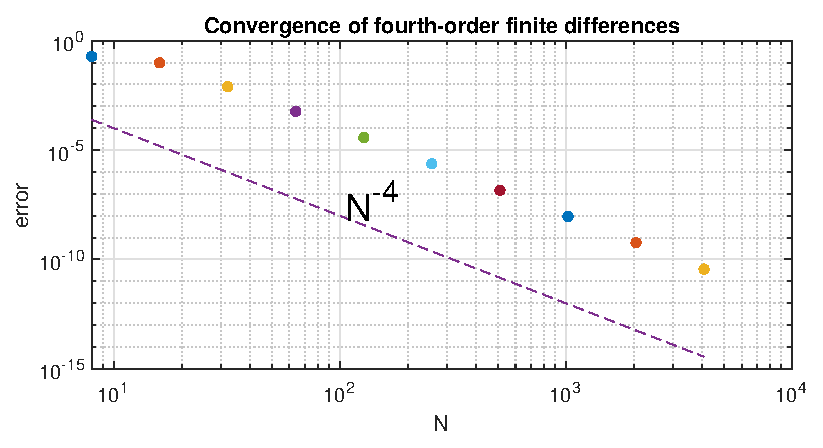
\includegraphics[]{p1a.eps}
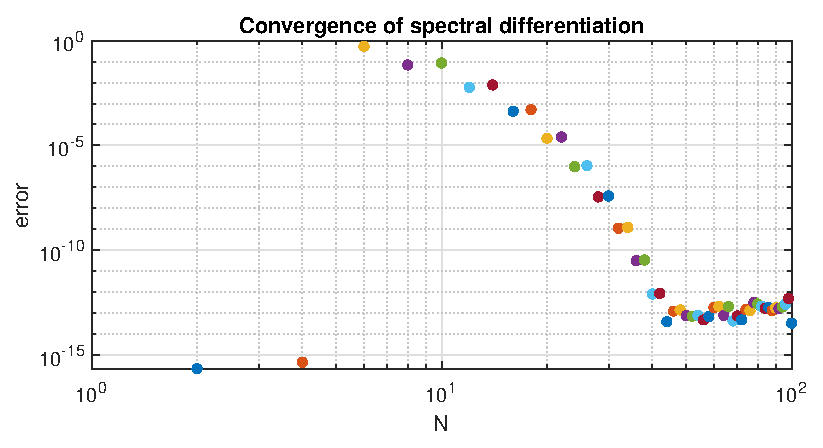
\includegraphics[]{p2a.eps}\\
We also obtain the following plots when the same programs are altered to take $u(x)=e^{\sin(x)|\sin(x)|}$:\\
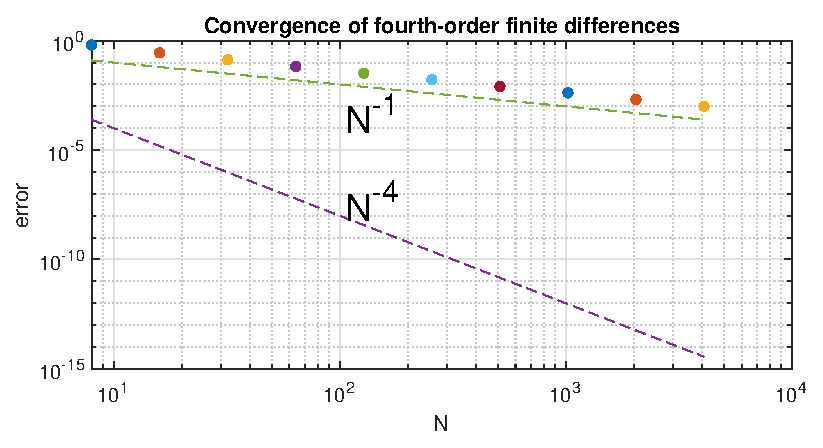
\includegraphics[]{p1b.eps}
\includegraphics[]{p2b.eps}\\
For the first function, we observe that fourth-order finite differences still roughly have $O(h^4)$ convergence and that spectral differentiation converges with spectral accuracy to machine precision. However, the second function appears to have roughly $O(h)$ convergence for both fourth-order finite differences and spectral differentiation. We know that we must have $O(h^4)$ and spectral convergence for sufficiently smooth functions, so one may suspect that $u(x)=e^{\sin(x)|\sin(x)|}$ is not sufficiently smooth. Indeed, one can use Wolfram-Alpha (or just plot $u'(x)=2|\sin(x)|\cos(x)e^{\sin(x)|\sin(x)|}$) to verify that its second derivative is discontinuous at zero which is likely the cause for the slower than expected convergence. 
\\See the attached .m files for the scripts that produce these plots. 
\section{Problem 4}
\subsection{Exercise 2.1}
Let $\mathcal{F}$ denote the Fourier transform operator defined such that $\mathcal{F}\{u\}(k)=\int_{-\infty}^\infty e^{-ikx}u(x)dx$ for any $u\in L^2(\real)$. Let $u,v\in L^2(\real)$ and $\hat{u},\hat{v}$ denote their respective Fourier transforms. We derive several properties of $\mathcal{F}$.
\subsubsection{Part a (linearity)}
Let $c$ be some constant.\\
\[
\begin{split}
\mathcal{F}\{u+v\}(k)&=\int_{-\infty}^\infty e^{-ikx}(u+v)(x)dx=\int_{-\infty}^\infty e^{-ikx}(u(x)+v(x))dx\\&=\int_{-\infty}^\infty e^{-ikx}u(x)dx+\int_{-\infty}^\infty e^{-ikx}v(x)dx=\hat{u}(k)+\hat{v}(k)
\end{split}
\]
\[
\mathcal{F}\{cu\}(k)=\int_{-\infty}^\infty e^{-ikx}(cu)(x)dx=\int_{-\infty}^\infty e^{-ikx}c(u(x))dx=c\int_{-\infty}^\infty e^{-ikx}u(x))dx=c\hat{u}(k).
\]
\subsubsection{Part b (translation)}
Let $x_0\in\real$. \\
\[
\mathcal{F}\{u(x+x_0)\}(k)=\int_{-\infty}^\infty e^{-ikx}u(x+x_0)dx
\]
We substitute $y=x+x_0$ (note $dy=dx$) to get 
\[
\mathcal{F}\{u(x+x_0)\}(k)=\int_{-\infty}^\infty e^{-ik(y-x_0)}u(y)dy=e^{ikx_0}\int_{-\infty}^\infty e^{-iky}u(y)dy=e^{ikx_0}\hat{u}(k).
\]
\subsubsection{Part e (conjugation)}
\[
\mathcal{F}\{\overline{u}\}(k)=\int_{-\infty}^\infty e^{-ikx}\overline{u}(x)dx = \int_{-\infty}^\infty \overline{\overline{e^{-ikx}}u(x)dx}= \int_{-\infty}^\infty \overline{e^{ikx}u(x)dx} = \overline{\int_{-\infty}^\infty e^{ikx}u(x)dx} = \overline{\hat{u}(-k)}
\]\\
Note that we can perform the penultimate step because $x$ is real. 
\subsubsection{Part f (differentiation)}
By the inverse Fourier transform, we have that 
\[
u(x)=\frac{1}{2\pi}\int_{-\infty}^\infty e^{ikx}\hat{u}(k)dk.
\]\\
Then, 
\[
\begin{split}
u_x(x)&=\frac{\partial }{\partial x}\bigg(\frac{1}{2\pi}\int_{-\infty}^\infty e^{ikx}\hat{u}(k)dk\bigg)=\frac{1}{2\pi}\int_{-\infty}^\infty \frac{\partial }{\partial x}(e^{ikx})\hat{u}(k)dk\\&=\frac{1}{2\pi}\int_{-\infty}^\infty ike^{ikx}\hat{u}(k)dk=\mathcal{F}^{-1}\{ik\hat{u}(k)\}.
\end{split}
\]\\
This yields that 
\[
\mathcal{F}\{u_x(x)\}=\mathcal{F}\{\mathcal{F}^{-1}\{ik\hat{u}(k)\}\}=ik\hat{u}(k).
\]
\subsection{Exercise 2.2}
\subsubsection{Part a}
Again, let $u\in L^2(\real)$ and let $\hat{u}$ denote its Fourier transform. We wish to show that $u(x)$ is even iff $\hat{u}(k)$ is even. \\
First, let $u(x)$ be even, i.e. $u(x)=u(-x)$ for any $x\in\real$. Then, we obtain the following by making a substitution $y=-x$ (note that $dy=-dx$).
\[
\begin{split}
\hat{u}(-k)&=\int_{-\infty}^\infty e^{-ikx}u(x)dx = \int_{\infty}^{-\infty} e^{iky}u(-y)(-dy)=\int_{-\infty}^{\infty} e^{iky}u(-y)(dy)\\&=\int_{-\infty}^{\infty} e^{iky}u(y)(dy)=\hat{u}(k).
\end{split}
\]
Thus, $\hat{u}(k)$ is also even.\\
Now, say that $\hat{u}(k)$ is even. Then, 
\[
\begin{split}
u(-x)&=\frac{1}{2\pi}\int_{-\infty}^{\infty}e^{-ikx}\hat{u}(k)dk=\frac{1}{2\pi}\int_{\infty}^{-\infty}e^{ilx}\hat{u}(-l)(-dl)=\frac{1}{2\pi}\int_{-\infty}^{\infty}e^{ilx}\hat{u}(-l)dl\\&=\frac{1}{2\pi}\int_{-\infty}^{\infty}e^{ilx}\hat{u}(l)dl=u(x).
\end{split}
\]
Note that we made the substitution $l=-k$. This gives that $u(x)$ is also even. Thus, $u(x)$ is even iff $\hat{u}(k)$ is even.\\
Now, we show that $u(x)$ is odd iff $\hat{u}(k)$ is odd in a very similar manner (the same substitutions will be performed to evaluate the integrals). \\
First, let u(x) be odd, i.e. $u(-x)=-u(x)$ for any $x\in\real$. Then, 
\[
\begin{split}
\hat{u}(-k)&=\int_{-\infty}^\infty e^{-ikx}u(x)dx = \int_{\infty}^{-\infty} e^{iky}u(-y)(-dy)=\int_{-\infty}^{\infty} e^{iky}u(-y)(dy)\\&=-\int_{-\infty}^{\infty} e^{iky}u(y)(dy)=-\hat{u}(k).
\end{split}
\]
Now, let $\hat{u}(k)$ be odd. Then, 
\[
\begin{split}
u(-x)&=\frac{1}{2\pi}\int_{-\infty}^{\infty}e^{-ikx}\hat{u}(k)dk=\frac{1}{2\pi}\int_{\infty}^{-\infty}e^{ilx}\hat{u}(-l)(-dl)=\frac{1}{2\pi}\int_{-\infty}^{\infty}e^{ilx}\hat{u}(-l)dl\\&=-\frac{1}{2\pi}\int_{-\infty}^{\infty}e^{ilx}\hat{u}(l)dl=-u(x).
\end{split}
\]
Thus, $u(x)$ is odd iff $\hat{u}(k)$ is odd.
\subsection{Exercise 2.4 (2.12 only)}
We wish to differentiate the sinc function $S_h(x)=\frac{\sin(\pi x/h)}{\pi x/h}$. Note that this formulation is not defined at $x=0$, but we let $S_h(0)=1$. For $x\neq0$, we differentiate
\[
S'_h(x)=\frac{(\pi x/h)(\pi/h)\cos(\pi x/h)-(\pi/h)\sin(\pi x/h)}{\pi^2x^2/h^2}=\frac{\cos(\pi x/h)}{x}-\frac{\sin(\pi x/h)}{\pi x^2/h}.
\]
If we take $x_j=jh$ and assume $j\neq0$, 
\[
S'_h(x_j)=\frac{\cos(\pi x_j/h)}{x_j}-\frac{\sin(\pi x_j/h)}{\pi x_j^2/h}=\frac{\cos(\pi j)}{jh}-\frac{\sin(\pi h)}{\pi j^2h}=\frac{(-1)^j}{jh}-\frac{0}{\pi j^2h}=\frac{(-1)^j}{jh}.
\]
To find the value of $S'_h(0)$, we consider the sinc function in its integral form $p(x)=\frac{h}{2\pi}\int_{-\pi/h}^{\pi/h}e^{ikx}dk$ and differentiate
\[
p'(x)=\frac{h}{2\pi}\int_{-\pi/h}^{\pi/h}\frac{\partial}{\partial x}(e^{ikx})dk=\frac{h}{2\pi}\int_{-\pi/h}^{\pi/h}ik(e^{ikx})dk
\]
Then,
\[
p'(0)=\frac{h}{2\pi}\int_{-\pi/h}^{\pi/h}ikdk=\frac{h}{2\pi}\left[\frac{ik^2}{2}\right]_{-\pi/h}^{\pi/h}=0.
\]
Thus, we can write 
\[
S'_h(x_j)= \begin{cases}
0, &j=0 \\
\frac{(-1)^j}{jh}, &j\neq0
\end{cases}
\]
\subsection{Exercise 2.7}
Modifying program 3 to determine the maximum error over $\real$ in the sinc function interpolants of the square wave and the hat function yields the following plot:\\
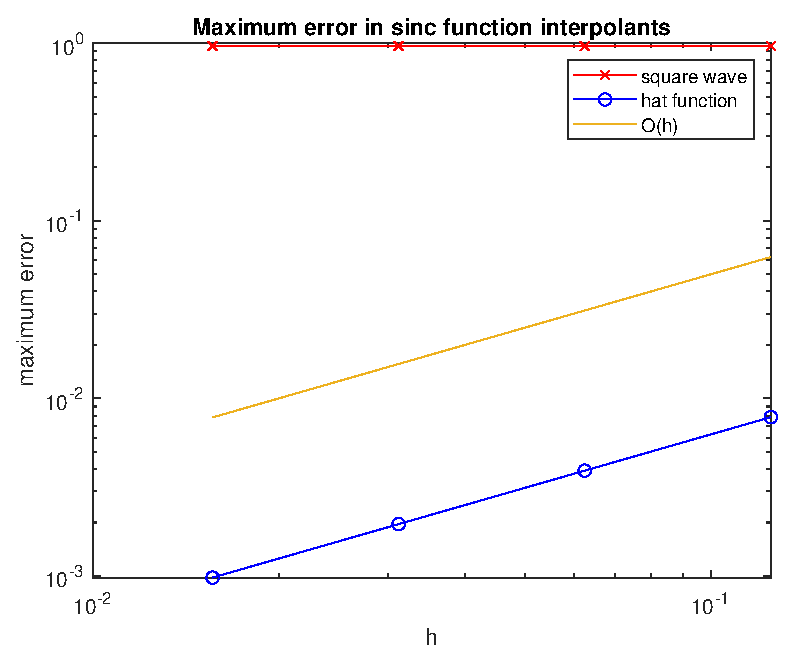
\includegraphics[]{p3.eps}
We can see that the error converges roughly linearly ($O(h)$) as h tends to 0 for the hat function. However, the error does not appear to converge at all for the square wave. This is likely due to the Gibbs phenomenon, because the square wave function is not sufficiently smooth in order to be accurately approximated by sinc interpolants. 
\end{document}
